\chapter{TINJAUAN PUSTAKA}
\label{chap:tinjauanpustaka}

% Ubah bagian-bagian berikut dengan isi dari tinjauan pustaka

\section{Penelitian Terdahulu}
\label{sec:penelitianterdahulu}

Penelitian-penelitian sebelumnya menggunakan beberapa metode AI untuk menyelesaikan masalah ini. Sebagian besar dari penelitian-penelitian sebelumnya berusaha untuk memperbaiki algoritma AI di game strategi seperti seri Civilization dalam sisi pembangunan kota atau ekonomi dalam game strategi. Namun, dalam sisi combat untuk game strategi masih belum diteliti.

I. Athaillah, S. M. S. Nugroho, dan M. Hariadi menggunakan Non-dominated Sorting Genetic Algorithm II (NGSA II) untuk optimasi pemilihan distrik kota dalam Civ6. Dibandingkan dengan metode AI yang ada dalam game tersebut, agen AI dalam simulasi penelitian ini dapat memberikan pemilihan distrik kota yang lebih optimal. Penelitian yang dilakukan oleh I. Athaillah, et al hanya berfokus pada pemilihan distrik dalam sebuah kota. Pemilihan distrik berpengaruh terhadap perkembangan ekonomi pemain. Metode NGSA II yang digunakan kurang cukup untuk mengatasi permasalahan dalam combat untuk AI. 

S. Wender dan I. Watson, menggunakan metode \emph{Q-Learning} untuk pemilihan bangunan kota dalam game Civilization IV. Performa agen AI dalam penelitian ini didapatkan lebih baik dibandingkan agen AI dalam game tersebut.

C. Amato dan G. Shani juga menggunakan sebuah metode \emph{Q-Learning} berupa \emph{Dyna-Q} dalam Civilization IV. Agen dalam penelitian ini didapatkan dapat beradaptasi terhadap lawan agen AI yang menggunakan \emph{fixed policy}.

Metode Reinforcement Learning yang digunakan oleh C. Amato dan G. Shani \citep{civ4RL}, serta S. Wender dan I. Watson kami rasa mencukupi untuk penelitian ini. Akan tetapi, game strategi Civilization IV yang dijadikan objek penelitian menggunakan desain game yang tidak lagi umum digunakan. Civilization IV menggunakan rectangular grid dibandingkan hexagonal grid yang banyak digunakan oleh game-game strategi berbasis giliran saat ini. Di dalam Civilization IV, tidak terdapat pembatasan \emph{unit} per tile yang banyak digunakan oleh game strategi saat ini. Tanpa batasan ini, pemain dapat melakukan \emph{doomstacking} dimana pemain dapat mengelompokan pasukan dalam satu tile sebanyak-banyaknya. Adanya \emph{doomstacking} membatasi pilihan strategi yang optimal dalam combat.

A. Sestini, et al \citep{deepCrawl} mengembangkan sebuah game bernama DeepCrawl yang menggunakan Deep Reinforcement Learning (DRL) sebagai metode untuk mengembangkan AI dalam game tersebut. AI yang dilatih dalam penelitian ini dapat memberikan tantangan yang cukup bagi banyak pemain.[5] Penggunaan DRL seperti yang digunakan oleh A. Sestini, et al pada game DeepCrawl merupakan metode yang paling optimal dalam game strategi. Penggunaan Neural Network (NN) dapat diskala untuk area game yang besar. Namun, DeepCrawl merupakan jenis game Roguelike yang sangat berbeda dan minim dibandingkan dengan game strategi 4X.

\section{Seri Game Civilization}
\emph{Civilization} merupakan seri \emph{turn-based strategy games} yang dirilis pada 1991. 
Game dari seri \emph{Civilization} telah menjual lebih dari 51 juta eksemplar \citep{civ6CopiesSold}.
Civilization juga biasa dikenal sebagai game 4X,
dimana pemain melakukan empat hal utama: \emph{explore}, \emph{expand}, \emph{exploit}, dan \emph{exterminate}. Secara makro, seluruh game
dalam seri \emph{Civilization} memiliki tema yang sama. Pemain dapat membangun, menggerakan \emph{unit}, dan melakukan negosiasi dengan pemain lain
berupa manusia maupun AI.

\begin{figure}[H]
  \centering
    % Nama dari file gambar yang diinputkan
    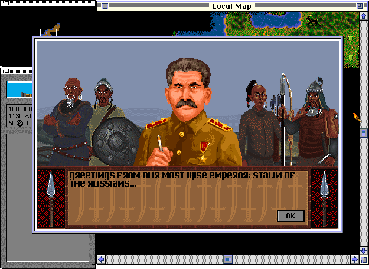
\includegraphics[scale=1]{gambar/Civ_1_negotiation.png}
    % Keterangan gambar yang diinputkan
    \caption{Layar negosiasi dalam \emph{Civilization} I.}
    % Label referensi dari gambar yang diinputkan
    \label{fig:civ1Negotiation}
\end{figure}

\emph{Civilization V} (Civ5) merupakan game pertama dalam seri ini untuk menggunakan \emph{hexagonal tile},
berbeda dengan game-game sebelumnya yang menggunakan \emph{square tile}. Civ5 juga membatasi posisi unit dengan peraturan \emph{one-unit-per-tile}
(1-UPT), dimana sebuah \emph{tile} hanya boleh ditempati oleh sebuah \emph{unit}.
Civ6 adalah game terbaru dalam seri ini. 

\section{Dasar Mekanisme Combat dalam Civilization VI}
Civ6 menggunakan \emph{hexagonal grid} yang terdiri dari \emph{hex tiles}, atau \emph{hexes}, sebagai basis pergerakan dan peletakan \emph{unit}. 
\emph{Unit} dapat bergerak ke enam arah menuju \emph{hexes} yang terdekat. Setiap \emph{unit} memiliki \emph{movement point} (MP). 
MP menentukan seberapa jauh \emph{unit} dapat bergerak atau melakukan aksi dalam satu giliran. 
Setiap pergerakan menuju \emph{hexes} lain akan mengurangi MP yang dimiliki \emph{unit} tersebut.
\emph{Unit} akan mendapatkan seluruh MP kembali setelah gilirannya selesai.

Saat \emph{combat}, \emph{unit} dapat memakan seluruh MP yang dimilikinya saat itu untuk menyerang \emph{unit} lain.
\emph{Unit} juga memiliki \emph{hit point} (HP), \emph{combat strength (CS)}, \emph{ranged strength} (RS), dan \emph{bombard strength} (BS).
CS digunakan ketika \emph{unit} menyerang \emph{unit} lain secara dekat, RS digunakan ketika \emph{unit} menyerang \emph{unit} lain menggunakan senjata jarak jauh, dan BS digunakan oleh \emph{siege} \emph{unit} ketika menyerang pertahanan kota.
\emph{Unit} yang diserang atau menyerang dengan CS akan mendapatkan \emph{damage} mengikuti persamaan eksponential\citep{civ6Combat}:

\[Damage(HP) = 30 * e^{(0.04+StrDiff)} * randomBetween(75\%, 125\%)\]

\emph{Unit} yang menerima \emph{damage} akan mendapatkan CS \emph{penalty} sebesar \(10 - HP/10\).
\emph{Unit} dapat mendapatkan kembali HP yang hilang (\emph{healing}) dengan cara tidak menggunakan MP yang dimiliki selama gilirannya.
\emph{Unit} yang melakukan \emph{healing} mendapatkan +10 HP per giliran.

\emph{Unit} jarak dekat (\emph{melee unit})  mempunyai \emph{Zone of Control} (ZoC). ZoC berada di lantai diseluruh sisi sebelah dimana 
\emph{unit} tersebut berada. Ketika sebuah unit memasuki ZoC milik unit lawan, unit tersebut tidak dapat bergerak ke lantai lain, namun
unit tersebut dapat melakukan aksi seperti menyerang dan sebagainya.

\section{Machine Learning}
\emph{Machine Learning} (ML) secara definisi merupakan suatu bidang ilmu komputer yang berkembang dari studi pengenalan pola dan teori pembelajaran komputasional dalam kecerdasan buatan. 
Prediksi dataset ML dibangun dari sebuah model yang mendapatkan contoh input untuk membuat prediksi berbasis data daripada mengikuti sebuah instruksi program statis \citep{machineL}.

\section{Reinforcment Learning}
\emph{Reinforcment Learning} (RL) merupakan pembelajaran dimana sebuah pembelajar (\emph{learner}) tidak diberitahu
secara eksplisit akan apa yang harus dilakukan, tetapi harus menemukan aksi (\emph{actions}) 
manakah yang akan memberikan imbalan (\emph{reward}) terbesar. 
RL berbeda akan paradigma ML yang lain seperti \emph{supervised learning} atau \emph{unsupervised learning} \citep{reinforcmentL}. 

\section{Deep Learning}
\emph{Deep Learning} merupakan bentuk dari \emph{machine learning} yang memungkinkan komputer untuk mempelajari pengalamannya dan memahami dunia secara konsep hierarkis. 
Konsep hierarkis ini memungkinkan komputer untuk mempelajari konsep rumit dengan membangun konsep tersebut dari konsep-konsep yang lebih sederhana \citep{deepL}.

\section{Deep Reinforcement Learning}
\emph{Deep Reinforcement Learning} (DRL) merupakan jenis dari \emph{Reinforcement Learning} (RL), dengan \emph{deep neural network} sebagai representasi state
dan/atau fungsi pendekatan untuk fungsi \emph{value}, \emph{policy}, \emph{transition model}, atau fungsi \emph{reward} \citep{deepRL}.
Sebuah environment game umum digunakan sebagai bidang eksperimentasi DRL.
\emph{DeepMind} membuat sebuah model DRL (\emph{AlphaStar}) yang dapat mengalahkan pemain professional dalam game \emph{Starcraft 2}, membuktikan bahwa DRL dapat digunakan untuk membangun agen AI yang mumpuni dalam sebuah game strategi \citep{alphaStar}.
\emph{OpenAI} juga mempresentasikan sebuah model yang dapat mengalahkan pemain professional dalam sebuah game \emph{Dota 2} \citep{openaiDota2}.
Penelitian-penelitian tersebut telah membuktikan kemampuan DRL dalam membuat sebuah agen AI yang mumpuni dalam game strategi.

\section{Deep Q-Learning Network}
Mnih, et al mengenalkan \emph{Deep Q-Learning Network} (DQN)\citep{deepQN} sebagai pencetus pertama metode \emph{Deep Reinforcement Learning}. DQN menggunakan \emph{neural network} untuk memperkirakan nilai optimal dari fungsi \emph{action value} pada \emph{Q-Learning}.
DQN, menggunakan \emph{experience replay} untuk mengatasi ketidakstabilan dan divergensi yang muncul pada \emph{Q-Learning} seperti, \emph{off-policy, function approximation,} dan \emph{bootstraping} \citep{deepQNFunction}.

DQN merepresentasikan sebuah fungsi \emph{action-value}:
\begin{equation}
  Q_*(s,a) = \sum_{s' \in \mathcal{S}, r\in\mathcal{R}}p(s',r|s,a)(r + \gamma \max_{a'\in\mathcal{A}(s')}Q_*(s',a'))
  \label{Eq:DQNEquation}
\end{equation}

Dimana $(s)$ merupakan keadaan setelah observasi dilakukan, sedangkan $(a)$ adalah aksi yang telah dilakukan sebelum observasi.
$(r)$ merupakan \emph{reward} yang didapatkan setelah melakukan aksi tersebut. Reward tersebut akan dikalikan dengan $(\gamma)$ atau \emph{discount}.

Saat pembelajaran, dilakukan \emph{Q-learning update} terhadap sampel (\emph{minibatches}) dari \emph{experience} $(s,a,r,s') \sim U(D)$
yang diambil secara acak dari sebuah kumpulan sampel. \emph{Q-learning update} dilakukan pada itersi i dan menggunakan fungsi \emph{loss}:

\begin{equation}
	\ell (\theta) = \mathbb E _{s, a, r, s'} \sim U(D) \left[r + 
    \gamma \max _{a'} Q (s', a';\theta^{-}_{i}) 
    - Q(s, a;\theta_{i})\right]^2
    \label{Eq:DQNLossFunction}
\end{equation}

$\gamma$ merupakan faktor \emph{discount}, $\theta$ merupakan parameter dari \emph{Q-network} pada iterasi i 
dan $\theta^{-}_{i}$ merupakan parameter \emph{target network} yang diupdate hanya dengan 
parameter \emph{Q-network} $(\theta_{i})$ pada setiap \emph{steps} $C$ \citep{deepQN}.

\begin{figure}[H]
  \centering
    % Nama dari file gambar yang diinputkan
    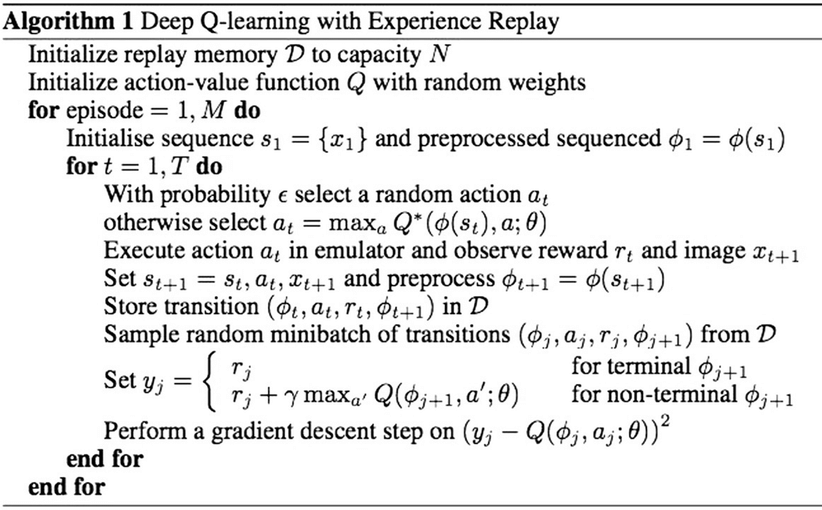
\includegraphics[scale=0.4]{gambar/dqn_algorithm.png}
    % Keterangan gambar yang diinputkan
    \caption{Algorithma \emph{Deep Q-Learning} \citep{deepQN}.}
    % Label referensi dari gambar yang diinputkan
    \label{fig:dqnAlgorithm}
\end{figure}

DQN memiliki kelemahan dimana perkiraan dari sebuah \emph{action value} nilainya terlalu besar.
DQN juga memiliki tendensi untuk mengejar \emph{action value} yang terbesar walau mungkin aksi tersebut tidaklah optimal pada situasi yang sedang dihadapi.
Melihat pada persamaan \ref{Eq:DQNEquation}, didapatkan $\max_{a'\in\mathcal{A}(s')}Q_*(s',a')$
yang mengambil nilai perkiraan maksimum secara implisit. Hal ini dapat menyebabkan \emph{maximization bias}
saat pembelajaran \cite{doubleQLearning}.

\emph{Double Deep Q-Learning} (DDQN) mencoba menstabilkan nilai \emph{action value} yang terlalu besar dengan menggunakan dua cabang \emph{hidden layer} pada DQN \citep{doubleDQN}.

\begin{figure}[H]
  \centering
    % Nama dari file gambar yang diinputkan
    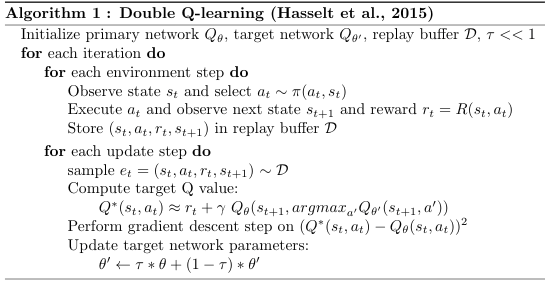
\includegraphics[scale=0.6]{gambar/ddqn_algorithm.png}
    % Keterangan gambar yang diinputkan
    \caption{Algoritma \emph{Double Deep Q-Learning} \citep{doubleDQN}.}
    % Label referensi dari gambar yang diinputkan
    \label{fig:ddqnAlgorithm}
\end{figure}

Algoritma DQN biasa melakukan \emph{uniform sampling} pada \emph{replay buffer} dimana
\emph{experience replay} diambil secara acak. Akan tetapi, hal ini dapat menyebabkan pengambilan sampel \emph{experience replay} yang kurang berguna pada saat pembelajaran.
Pada \emph{Prioritized Experience Replay} (PER), \emph{experience replay} yang lebih penting dalam
pembelajaran akan diambil lebih sering.
Prioritas ini didapatkan dengan mengithung nilai \emph{TD-error} \citep{prioritizedER}:

\begin{equation}
  \delta_{i} = r_{t} + \gamma \max_{a\in\mathcal{A}}Q_{\theta ^{-}}(s_{t+1},a) - Q_{\theta}(s_{t},a_{t})
  \label{Eq:DQNTDErrorEquation}
\end{equation}
atau pada \emph{Double} DQN:

\begin{equation}
  \delta_{i} = r_{t} + \gamma Q_{\theta^{-}} \left(s_{t+1}, \text{argmax}_{a\in\mathcal{A}}Q_{\theta ^{-}}(s_{t+1},a)\right) - Q_{\theta}(s_{t},a_{t}) 
  \label{Eq:DDQNTDErrorEquation}
\end{equation}

\begin{figure}[H]
  \centering
    % Nama dari file gambar yang diinputkan
    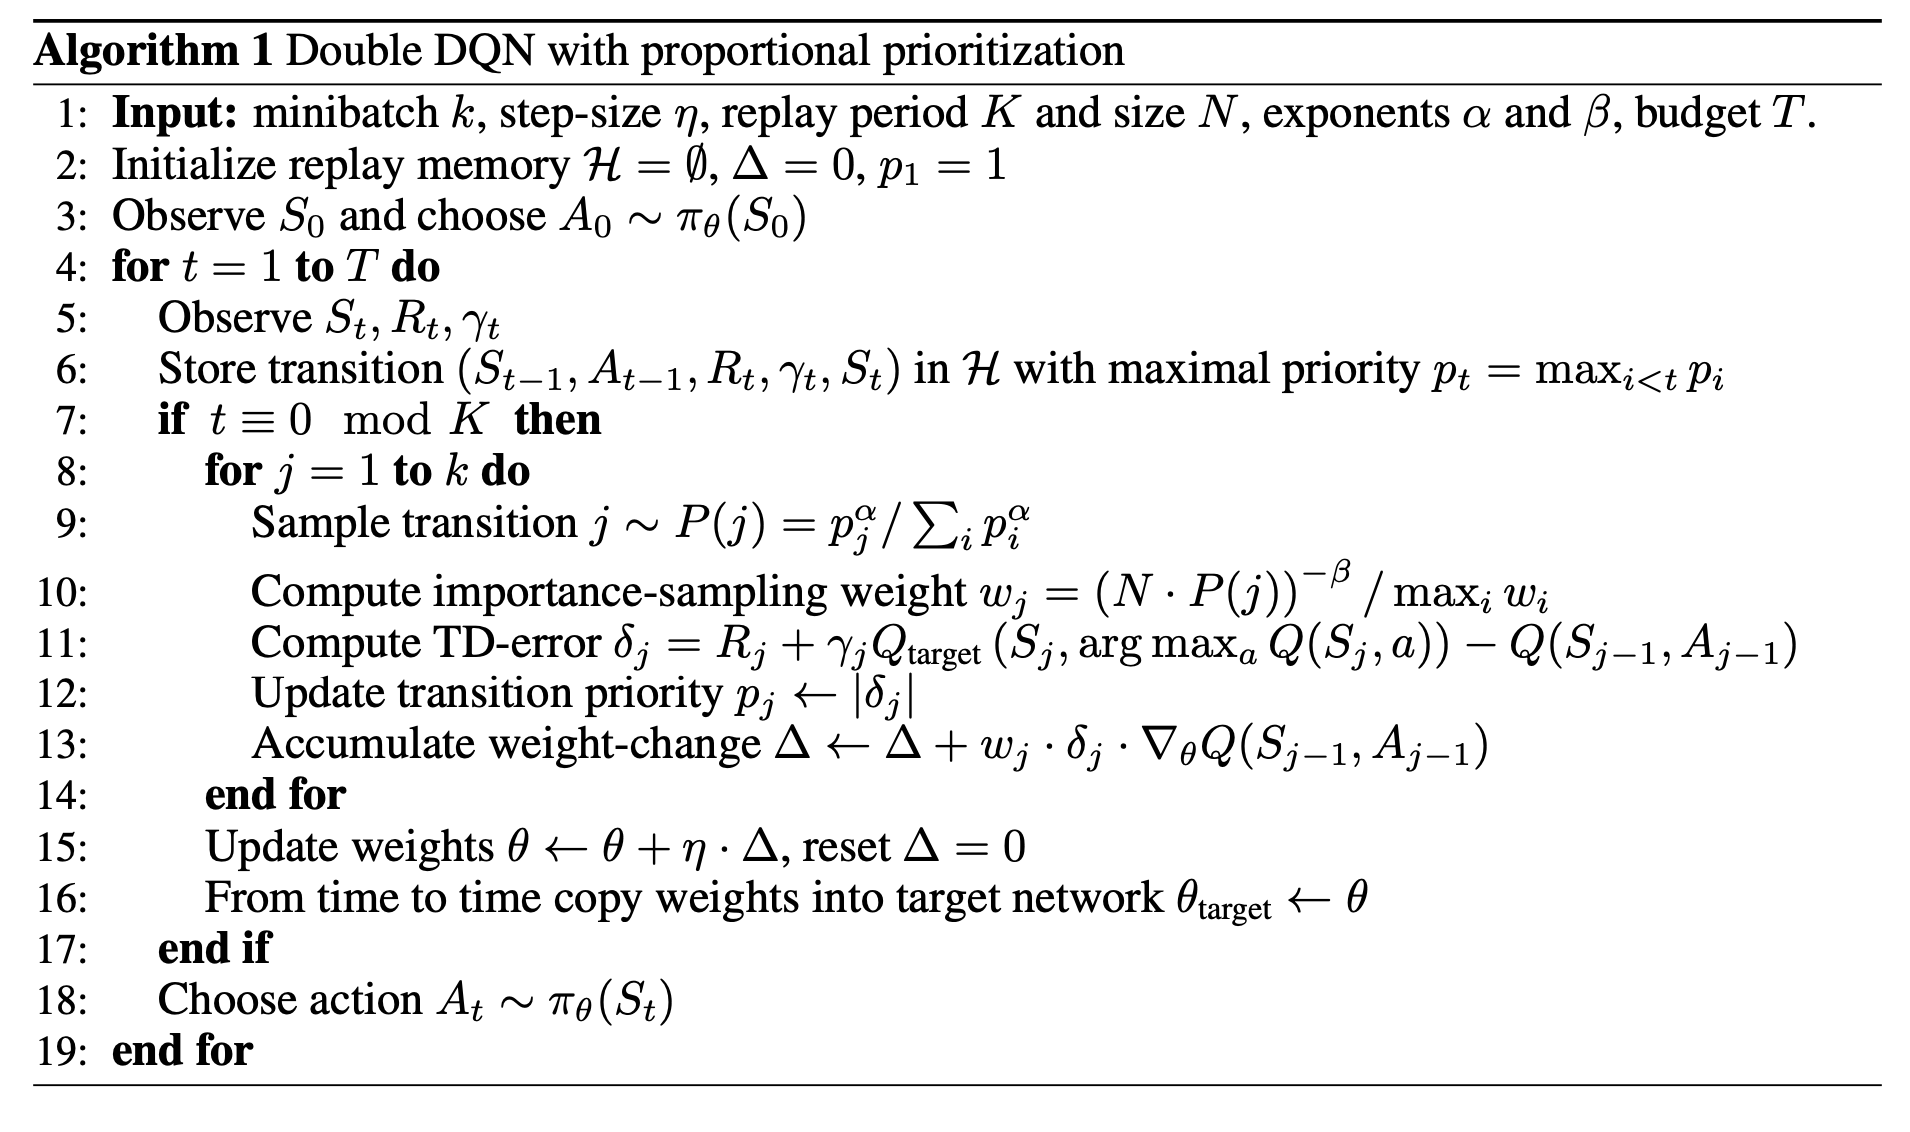
\includegraphics[scale=0.4]{gambar/ddqn_per_algorithm.png}
    % Keterangan gambar yang diinputkan
    \caption{Algorithma \emph{Double Deep Q-Learning} dengan \emph{Prioritized Experience Replay} \citep{prioritizedER}.}
    % Label referensi dari gambar yang diinputkan
    \label{fig:dqnPerAlgorithm}
\end{figure}

\emph{Dueling} DQN memisahkan neural network menjadi dua bagian, satu bagian mempelajari dan memberikan estimasi nilai pada seluruh \emph{timestep},
dan bagian lain menghitung nilai potensial (\emph{advantage}) dari sebuah aksi.
Kedua bagian ini digabungkan menjadi satu \emph{action-advantage Q function} \citep{duelingDQN}.

\begin{figure}[H]
  \centering
    % Nama dari file gambar yang diinputkan
    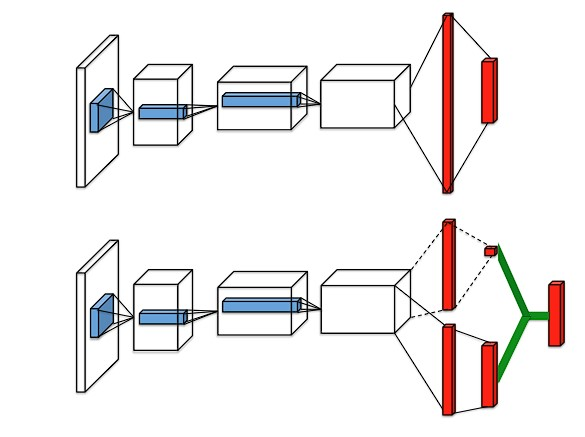
\includegraphics[scale=0.5]{gambar/dqn_vs_dueling_dqn_architecture.jpg}
    % Keterangan gambar yang diinputkan
    \caption{Arsitektur DQN (di atas) dibandingkan dengan Arsitektur \emph{Dueling} DQN (di bawah)}
    % Label referensi dari gambar yang diinputkan
    \label{fig:dqnVsDuelingDqnArchitecture}
\end{figure}

\section{Distributed Prioritized Experience Replay Deep Q-Networks (APE-X DQN)}

Distributed Prioritized Experience Replay Deep Q-Networks (Ape-X DQN) merupakan arsitektur DQN terdistribusi.
Dibandingkan dengan DQN biasanya, Ape-X DQN menggunakan banyak \emph{core} pada CPU sebagai \emph{actor} yang masing masing memiliki environment tersendiri.
\emph{Actor} tersebut akan mengumpulkan \emph{experience} yang didapatkan ke sebuah GPU \emph{learner}. 
\emph{Learner} tersebut akan mengambil sebuah sampel dengan metode \emph{prioritized experience} dan melakukan update pada \emph{neural network}. 
APE-X DQN ditemukan lebih efisien dan lebih baik daripada algoritma DQN lainnya dalam \emph{environment} game \emph{Atari} 2600 \citep{apexDQN}.

\begin{figure}[H]
  \centering
    % Nama dari file gambar yang diinputkan
    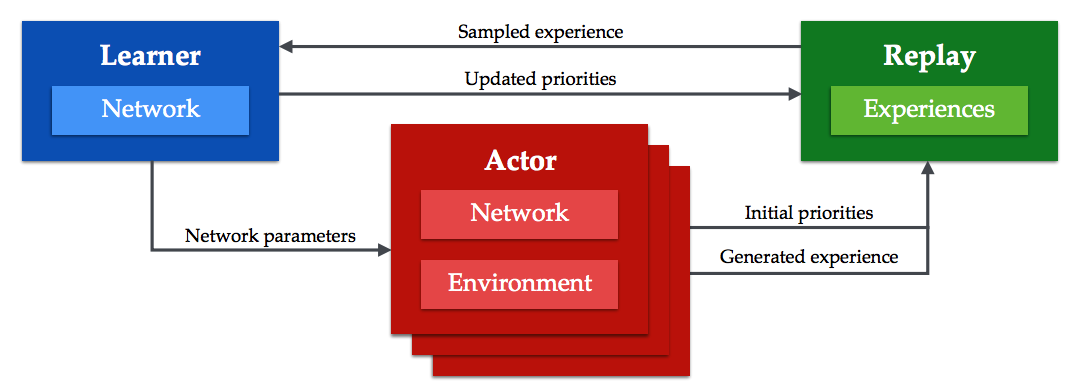
\includegraphics[scale=0.6]{gambar/apex1.png}
    % Keterangan gambar yang diinputkan
    \caption{Arsitektur APE-X dengan beberapa \emph{actor} dan menambahkan \emph{experiences} ke pada sebuah \emph{learner} \citep{apexDQN}.}
    % Label referensi dari gambar yang diinputkan
    \label{fig:apexDQNArchitecture}
\end{figure}

APE-X DQN memiliki seuah fungsi \emph{loss} untuk menghitung seluruh elemen dari \emph{batch} sebagai berikut:
\begin{equation}
  l_{t} (\theta) = \frac{1}{2}\left(G_{t}-q\left(S_{t},A_{t},\theta\right)\right)^2
\end{equation}
dengan 
\begin{equation}
  G_{t} = R_{t+1} + \gamma R_{t+2} + \dots + \gamma ^{n-1}R_{t+n} + \gamma ^{n}q\left(S_{t+n}, \text{argmax} q\left(S_{t+n},a,\theta \right)\theta ^{-}\right)
\end{equation}
dimana $t$ merupakan indeks dari \emph{experience} yang diambil dari \emph{replay} dimulai dari \emph{state} $S_{t}$ dan \emph{action} $A_{t}$,
dan $\theta^{-}$ menandakan parameter dari \emph{target network} \citep{apexDQN}.

\section{Proximal Policy Optimization}

\emph{Proximal Policy Optimization} (PPO) merupakan sebuah \emph{Policy Gradient Methods}. 
Berbeda dengan \emph{Q-Learning}, \emph{policy gradient methods} bekerja dengan cara menghitung sebuah estimator dari \emph{policy gradient} dan memasukannya ke
sebuah algoritma \emph{stochastic gradient ascent} \citep{ppo}. PPO mengoptimasi lebih lanjut dari mode \emph{Trust Region Policy Optimization} (TRPO).
Jika biasanya metode \emph{policy-gradient} melakukan satu \emph{gradient update} setiap sampel, PPO melakukan beberapa \emph{epochs} dari \emph{minibatch updates}. 
PPO memiliki beberapa keuntungan dari TRPO dengan implementasi yang lebih mudah, lebih baik dalam generalisasi, 
dan memiliki performa yang lebih baik dalam simulasi permainan game Atari dibandingkan dengan metode policy gradient yang lain.

PPO melakukan optimasi \emph{trust region} dengan mengganti batasan dari \emph{penalty} dalam sebuah fungsi \emph{objective}:
\begin{equation}
  L^{KLPEN} (\theta) = \mathbb{\hat{E}}\left[\frac{\pi_{\theta} (a_{t} | s_{t})}{\pi_{\theta_{old}} (a_{t} | s_{t})}\right] \hat{A}_{t} - \beta KL \left[\pi_{\theta_{old}}(. | s_{t}), \pi \theta(. | s_{t})\right]
\end{equation}
$\beta$ mengurangi \emph{objective} ketika sebuah \emph{policy} baru berbeda dengan \emph{policy} lama.
Jika \emph{KL-divergence} dari \emph{policy} baru dan lama lebih tinggi dari nilai target,
nilai $\beta$ akan dikurangi. Sebaliknya, jika nilai tersebut dibawah nilai target, maka nilai $\beta$ akan bertambah.

Pendekatan lain adalah menggunakan \emph{clipped surrogate objective}:
\begin{equation}
  L^{CLIP} (\theta) = \mathbb{\hat{E}}_{t}\left[\text{min}(r_{t}{\theta}\hat{A}_{t},\text{clip}(r_{t}(\theta),1-\epsilon,1+\epsilon)\hat{A}_{t})\right]
\end{equation}
dimana \emph{epsilon} adalah \emph{hyperparameter}. 
Saat rasio probabilitas dari \emph{policy} lama dan baru berada di luar ($1-\epsilon$) dan ($1+\epsilon$),
fungsi \emph{advantage} akan dipotong nilainya (\emph{clipped}). 
Dengan memotong nilai advantage, perubahan \emph{policy} yang diluar set \emph{hyperparameter} akan tidak sering terjadi, 
menjadikan proses \emph{update} lebih stabil.

\begin{figure}[H]
  \centering
    % Nama dari file gambar yang diinputkan
    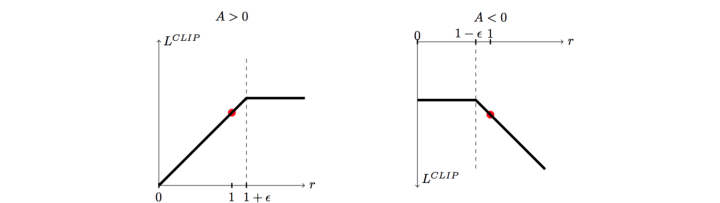
\includegraphics[scale=0.6]{gambar/ppo_clipped.png}
    % Keterangan gambar yang diinputkan
    \caption{Plot menunjugan sebuah timestep dari fungsi \emph{surrogate} $L^{CLIP}$
    sebagai fungsi rasio probabilitas. \emph{Advantage} positif (kiri) dan \emph{advantage} negatif (kanan).
    Lingkaran merah menunjukan titik awal untuk optimasi.}
    % Label referensi dari gambar yang diinputkan
    \label{fig:ppoClippedPlot}
\end{figure}

\section{Importance Weighted Actor-Learner Architecture (IMPALA)}

IMPALA merupakan sebuah \emph{framework} \emph{actor-critic} yang memisahkan antara acting dengan learning.
IMPALA menggunakan \emph{V-trace} dimana \emph{learner} mempelajari \emph{experience trajectory}.
GPU \emph{learner} pusat melakukan \emph{stochastic gradient descent} (SGD) pada sebuah \emph{tight loop} saat mengambil sampel 
\emph{batches} dari proses CPU \emph{actor} secara asinkronus \citep{impala}.

\emph{V-trace} merupakan sebuah algoritma RL \emph{off-policy actor-critic} yang mengurangi \emph{lag} dari \emph{actions} yang dibuat oleh \emph{actors}
dan saat \emph{learner} melakukan estimasi \emph{gradient}. 
Pada sebuah \emph{trajectory} $(x_{t}, a_{t}, r_{t})^{t=s+n}_{t=s}$ yang dibuat oleh \emph{actor} yang mengikut sebuah \emph{policy} $\mu$.
Target \emph{V-trace} pada \emph{$n$-steps} untuk $V(x_{s})$, dnegan nilai perkiraan pada \emph{state} $x_{s}$ di definisikan sebagai:
\begin{equation}
  v_{s} \stackrel{\text{def}}{=} V(x_{s}) + \sum^{s+n-1}_{t=s} \gamma^{t-s} \left(\Pi^{t-1}_{i=s}ci\right) \delta_{t}V
\end{equation}
dimana $\delta_{t}V \stackrel{\text{def}}{=} \rho_{t}\left(r_{t} + \gamma V(x_{t+1}) - V(x_{t})\right)$ merupakan perbedaan temporal untuk $V$,
dan $\rho_{t} \stackrel{\text{def}}{=} \text{min}\left(\overline{\rho}, \frac{\pi (a_{t}|x_{t})}{\mu (a_{t}|x_{t})}\right)$ dan 
$c_{i} \stackrel{\text{def}}{=} \text{min}\left(\overline{c}, \frac{\pi (a_{t}|x_{t})}{\mu (a_{t}|x_{t})}\right)$ adalah \emph{truncated importance sampling weight}.
Diasumsikan juga bahwa nilai \emph{truncation levels} adalah $\overline{\rho} \geq \overline{c}$ \citep{impala}.

Arsitektur IMPALA dapat mencapai \emph{throughput} yang tinggi, namun \emph{policy} yang digunakan untuk menghasilkan \emph{trajectory} terlambat selama beberapa \emph{update} jika dibandingkan dengan \emph{policy} yang ada pada \emph{learner} pada saat perhitungan gradien.
Oleh karena itu, IMPALA menggunakan \emph{V-trace off policy actor critic}

\begin{figure}[H]
  \centering
    % Nama dari file gambar yang diinputkan
    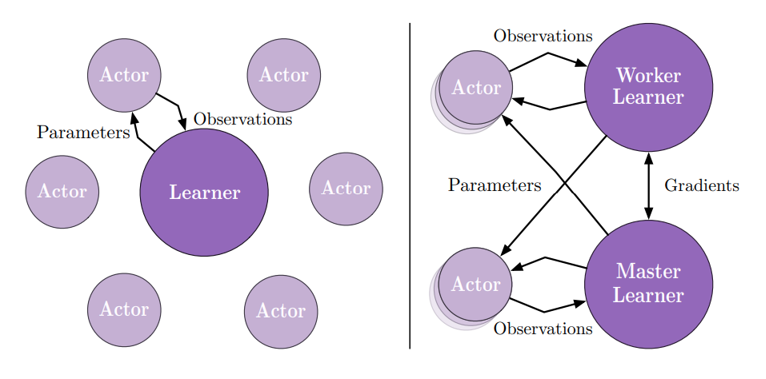
\includegraphics[scale=0.8]{gambar/impala_worker.png}
    % Keterangan gambar yang diinputkan
    \caption{Kiri: Sebuah learner. Setiap \emph{actor} menghasilkan \emph{trajectories} dan mengirimkannya melalui sebuah \emph{queue} kepada \emph{learner}.
    Sebelum memulai \emph{trajectory} selanjutnya, \emph{actor} menerima \emph{policy parameters} terbaru dari \emph{learner}.
    Kanan: Banyak \emph{learner}. \emph{Policy parameters} didistribusikan kepada lebih dari satu \emph{learner} yang bekerja secara sinkronus \citep{impala}.}
    % Label referensi dari gambar yang diinputkan
    \label{fig:impalaSingleVsMultipleLearner}
\end{figure}

\section{PettingZoo}

PettingZoo merupakan sebuah \emph{library} untuk membuat \emph{environment} yang mendukung \emph{multi agent reinforcement learning} (MARL).
PettingZoo menggunakan sebuah model formal \emph{game environment} baru yang disebut \emph{Agent Environment Cycle} (AEC). Dalam AEC, agen akan secara sekuensial melakukan \emph{observations}, mengambil \emph{actions}, mendapatkan \emph{rewards} yang diberikan dari agen lain, dan kemudian agen berikutnya melakukan \emph{actions}.
Model ini sangat cocok untuk game berbasis giliran \citep{pettingZoo}.

\begin{figure}[H]
  \centering
    % Nama dari file gambar yang diinputkan
    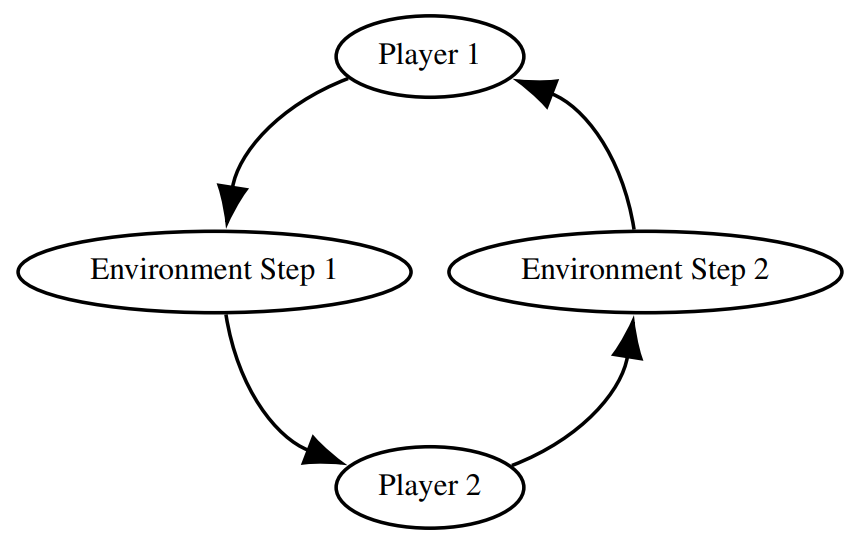
\includegraphics[scale=0.5]{gambar/actor_environment_cycle.png}
    % Keterangan gambar yang diinputkan
    \caption{Diagram AEC pada \emph{environment} dengan dua agen seperti catur}
    % Label referensi dari gambar yang diinputkan
    \label{fig:actorEnvironmentCycle}
\end{figure}

PettingZoo memiliki API yang mirip dengan Gym. Kemiripan API ini memudahkan pengguna untuk menggunakan ataupun mengubah \emph{library environment} dari Gym ke PettingZoo ataupun sebaliknya.

% Contoh pembuatan potongan kode
\begin{lstlisting}[
  language=Python,
  caption={Contoh dasar penggunaan API Gym.},
  label={lst:gymAPI}
]
  import gym
  env = gym.make('CartPole-v0')
  observation = env.reset()
  for _ in range(1000):
  action = policy(observation)
  observation, reward, done, info = env.step(action)
\end{lstlisting}

\begin{lstlisting}[
  language=Python,
  caption={Contoh dasar penggunaan API PettingZoo.},
  label={lst:pettingZooAPI}
]
  from ray.rllib.examples.env.multi_agent
  import MultiAgentCartPole
  env = MultiAgentCartPole()
  observation = env.reset()
  for _ in range(1000):
  actions = policies(agents, observation)
  observation, rewards, dones,
  infos = env.step(actions)
\end{lstlisting}

\section{RLlib}
RLlib adalah sebuah \emph{library} RL yang merupakan bagian dari \emph{open source Ray project} yang menawarkan
algoritma RL berskala dan performa tinggi untuk komputasi terdistribusi \citep{rllib}.
RLlib menawarkan beberapa koleksi dan referensi algoritma dan juga abstraksi \emph{scalable} untuk memudahkan
pembuatan algoritma baru. RLlib mendukung beberapa \emph{library} \emph{environment} seperti \emph{OpenAI Gym},
\emph{PettingZoo}, dan juga simulator eksternal seperti \emph{Unity3D} atau \emph{game engine} lainnya \citep{rllibDocumentation}.